% 二阶行列式的对角线法则
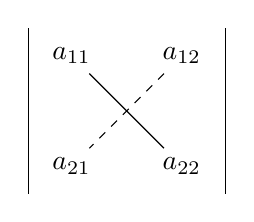
\begin{tikzpicture}
  \draw (-1.25,1.05) -- (-1.25,-1.05);

  \node at (-.7,.7) (a11) {$a_{11}$};
  \node at (.7,-.7) (a22) {$a_{22}$};
  \draw (a11) -- (a22);

  \node at (.7,.7) (a12) {$a_{12}$};
  \node at (-.7,-.7) (a21) {$a_{21}$};
  \draw[dashed] (a12) -- (a21);

  \draw (1.25,1.05) -- (1.25,-1.05);
\end{tikzpicture}
